%%% UNIT 3
{
\setbeamertemplate{headline}{}
\setbeamertemplate{footline}{
  \begin{beamercolorbox}[wd=\paperwidth,ht=2.2ex,dp=1.5ex]{palette quaternary}
  \end{beamercolorbox}
  }
\begin{frame}[noframenumbering]
\frametitle{\DB{\huge{\textbf{$\blacksquare$ Unit 3}}}}
\myPause
 \begin{itemize}
 \item[] \LARGE{\MB{Practice session 1}}
 \item[] \vspace{-1mm}\hspace{5mm}\Large{\MB{Dynamic systems}}
 \end{itemize}
\end{frame}
}

\part{}

\section{Exercise 01}
\subsection{}

\begin{frame}
\frametitleTC{Problem}
\framesubtitleTC{This one we solve together}
\myPause
 Given the DT LTI dynamic system described in the state space by
 \begin{displaymath}
  A = \begin{bmatrix} 0.4 & 0.4 \\ 0.05 & 0.3 \end{bmatrix}, \quad
  b = \begin{bmatrix} 1 \\ 0.5 \end{bmatrix}, \quad
  c = \begin{bmatrix} 2 & -1 \end{bmatrix}, \quad
  d = 0,
 \end{displaymath}
 \begin{itemize}[<+-| alert@+>]
 \item[(a)] discuss its stability,
 \item[(b)] express it in scalar form,
 \item[(c)] compute its transfer function,
 \item[(d)] compute the first three values ($k=0,1,2$) of its response to
            \begin{displaymath}
             x(0) = \begin{bmatrix} 2 \\ 1 \end{bmatrix}, \quad
             u(k) = 0.4k.
            \end{displaymath}
 \end{itemize}
\end{frame}

\begin{frame}
\frametitleTC{Solution}
\framesubtitleTC{Item (a)}
\myPause
 \begin{itemize}[<+-| alert@+>]
 \item We need to compute the eigenvalues $\lambda_{1,2}$ of $A$:
       \begin{itemize}[<+-| alert@+>]
       \item[] \vspace{1mm}
               $\det(\lambda I -A) = 0$,
       \item[] \vspace{1mm}
               $\det \left(
                     \begin{bmatrix} \lambda & 0 \\ 0 & \lambda \end{bmatrix}
                    -\begin{bmatrix} 0.4 & 0.4 \\ 0.05 & 0.3 \end{bmatrix}
                     \right) = 0 $,
       \item[] \vspace{1mm}
               $\det \begin{bmatrix} \lambda-0.4 & -0.4 \\
                                    -0.05       & \lambda-0.3 \end{bmatrix} = 0 $,
       \item[] \vspace{1mm}
               $(\lambda-0.4)(\lambda-0.3)-(-0.4)(-0.05) = 0$,
       \item[] \vspace{1mm}
               $\lambda^2-0.7\lambda+0.1=0$,
       \item[] \vspace{1mm}
               $\lambda=\cfrac{0.7\mp\sqrt{0.7^2-4\cdot 0.5}}{2} \quad \Rightarrow \quad
                \lambda_1=0.2, \; \lambda_2=0.5.$
       \end{itemize}
 \item All the eigenvalues of $A$ are strictly less than one in magnitude\\
       $\Rightarrow$ the system is asymptotically stable.
 \end{itemize}
\end{frame}

\begin{frame}
\frametitleTC{Solution}
\framesubtitleTC{Item (b)}
\myPause
 \begin{itemize}[<+-| alert@+>]
 \item Denoting by $x=[x_1\;x_2]'$ the state vector (sign $'$means transpose) we have
       \begin{displaymath}
        \left\{\begin{array}{rcl}
         \begin{bmatrix} x_1(k) \\ x_2(k) \end{bmatrix} 
         &=&             
         \begin{bmatrix} 0.4 & 0.4 \\ 0.05 & 0.3 \end{bmatrix}\,
         \begin{bmatrix} x_1(k-1) \\ x_2(k-1) \end{bmatrix}
         +
         \begin{bmatrix} 1 \\ 0.5 \end{bmatrix}\,
         u(k-1) \\
         y(k)
         &=&          
         \begin{bmatrix} 2 & -1 \end{bmatrix} \,
         \begin{bmatrix} x_1(k) \\ x_2(k) \end{bmatrix}
        \end{array}\right.
       \end{displaymath}
 \item hence in scalar form
       \begin{displaymath}
        \left\{\begin{array}{rcl}
         x_1(k) &=&  0.4 x_1(k-1) + 0.4 x_2(k-1) +    u(k-1)\\
         x_2(k) &=& 0.05 x_1(k-1) + 0.3 x_2(k-1) + 0.5u(k-1)\\
         y(k)   &=&    2 x_1(k-1) -     x_2(k-1)
        \end{array}\right.
       \end{displaymath}
 \end{itemize}
\end{frame}

\begin{frame}
\frametitleTC{Solution}
\framesubtitleTC{Item (c)}
\myPause
 \begin{itemize}[<+-| alert@+>]
 \item The transfer function $G(z)$ is $c(zI-A)^{-1}b+d$, hence
       \begin{itemize}
       \item[] \begin{itemize}[<+-| alert@+>]
               \item[$G(z)$] \vspace{1mm}
                    $= \begin{bmatrix} 2 & -1 \end{bmatrix} \,
                       \begin{bmatrix} z-0.4 & -0.4 \\
                       -0.05& z-0.3 \end{bmatrix}^{-1} \,
                       \begin{bmatrix} 1 \\ 0.5 \end{bmatrix}
                       +0
                    $
               \item[] \vspace{1mm}
                    $= \cfrac{1}{(z-0.5)(z-0.2)}
                       \begin{bmatrix} 2 & -1 \end{bmatrix} \,
                       \begin{bmatrix} z-0.3 & 0.4 \\
                       0.05& z-0.4 \end{bmatrix} \,
                       \begin{bmatrix} 1 \\ 0.5 \end{bmatrix}
                    $
               \item[] \vspace{1mm}
                    $= \cfrac{1}{(z-0.5)(z-0.2)}
                       \begin{bmatrix} 2z-0.65 &-z+1.2 \end{bmatrix} \,
                       \begin{bmatrix} 1 \\ 0.5 \end{bmatrix}
                    $
               \item[] \vspace{1mm}
                    $= \cfrac{1.5z-0.05}{(z-0.5)(z-0.2)}.
                    $
               \end{itemize}
       \end{itemize}
 \end{itemize}
\end{frame}

\begin{frame}
\frametitleTC{Solution}
\framesubtitleTC{Item (d)}
\myPause
 \begin{itemize}[<+-| alert@+>]
 \item We have\\
       $u(0) = 0, \quad u(1) = 0.4, \quad u(2) = 0.8, \quad u(3) = 1.2, \, \ldots$
 \item We need to iteratively apply the state and output equations, whence
       \begin{itemize}
       \item[] \begin{itemize}[<+-| alert@+>]
               \item[$k=0$:] \vspace{1mm} 
                    $\left\{\begin{array}{rll}
                     x(0) &= \begin{bmatrix} 2 \\ 1 \end{bmatrix} (\text{given}) \\
                     y(0) &= \begin{bmatrix} 2 & -1 \end{bmatrix} \,
                             \begin{bmatrix} 2 \\ 1 \end{bmatrix}
                          &= 3
                     \end{array}\right.
                    $
               \item[$k=1$:] \vspace{1mm} 
                    $\left\{\begin{array}{rll}
                     x(1) &= \begin{bmatrix} 0.4 & 0.4 \\ 0.05 & 0.3 \end{bmatrix} \,
                             \begin{bmatrix} 2 \\ 1 \end{bmatrix}
                            +\begin{bmatrix} 1 \\ 0.5 \end{bmatrix} \cdot 0
                          &= \begin{bmatrix} 1.2 \\ 0.4 \end{bmatrix}\\
                     y(1) &= \begin{bmatrix} 2 & -1 \end{bmatrix} \,
                             \begin{bmatrix} 1.2 \\ 0.4 \end{bmatrix}
                          &= 2
                     \end{array}\right.
                    $
               \item[$k=2$:] \vspace{1mm} 
                    $\left\{\begin{array}{rll}
                     x(1) &= \begin{bmatrix} 0.4 & 0.4 \\ 0.05 & 0.3 \end{bmatrix} \,
                             \begin{bmatrix} 1.2 \\ 0.4 \end{bmatrix}
                            +\begin{bmatrix} 1 \\ 0.5 \end{bmatrix} \cdot 0.4
                          &= \begin{bmatrix} 1.04 \\ 0.38 \end{bmatrix}\\
                     y(1) &= \begin{bmatrix} 2 & -1 \end{bmatrix} \,
                             \begin{bmatrix} 1.04 \\ 0.38 \end{bmatrix}
                          &= 1.7
                     \end{array}\right.
                    $
               \end{itemize}
       \end{itemize}
 \end{itemize}
\end{frame}

\begin{frame}
\frametitleTC{Addendum}
\framesubtitleTC{}
\myPause
 \begin{itemize}[<+-| alert@+>]
 \item We define some signals useful for the following.
       \begin{itemize}[<+-| alert@+>]
       \item Impulse (precisely, \TC{unit} impulse as the value is 1):
             \begin{displaymath}
              imp(k) = \begin{cases} 1 & k=0 \\ 0 & \text{otherwise} \end{cases}
             \end{displaymath}
       \item Step (\TC{unit} step, amplitude is 1):
             \begin{displaymath}
              step(k) = \begin{cases} 1 & k \geq 0 \\ 0 & \text{otherwise} \end{cases}
             \end{displaymath}
       \item Ramp(\TC{unit} ramp, slope is 1):
             \begin{displaymath}
              ramp(k) = k\; step(k) = \begin{cases} k & k \geq 0 \\ 0 & \text{otherwise} \end{cases}
             \end{displaymath}
       \end{itemize}
 \item Quite frequently ``unit'' is omitted, e.g. ``step response'' actually\\
       means ``unit step response''.
 \end{itemize}
\end{frame}

\begin{frame}
\frametitleTC{Proposed exercise 01}
\framesubtitleTC{Try this at home, ask questions next time if needed}
\myPause
 Given the DT LTI dynamic system described in the state space by
 \begin{displaymath}
  A = \begin{bmatrix} 0.5 & 0 \\ 2 & -0.3 \end{bmatrix}, \quad
  b = \begin{bmatrix} 1 \\ 0 \end{bmatrix}, \quad
  c = \begin{bmatrix} 0 & 4 \end{bmatrix}, \quad
  d = 1,
 \end{displaymath}
 \begin{itemize}[<+-| alert@+>]
 \item[(a)] discuss its stability,
 \item[(b)] express it in scalar form,
 \item[(c)] compute its transfer function,
 \item[(d)] compute the first three values ($k=0,1,2$) of its response to
            \begin{displaymath}
             x(0) = \begin{bmatrix} 1 \\ 1 \end{bmatrix}, \quad
             u(k) = 2 step(k).
            \end{displaymath}
 \end{itemize}
\end{frame}

\begin{frame}[fragile]
\frametitleTC{But how can we check our results?}
\framesubtitleTC{}
\myPause
 \begin{itemize}[<+-| alert@+>]
 \item With the symbolic package wxMaxima:
       \begin{verbatim}
        A  : matrix([0.4,0.4],[0.05,0.3]);
        b  : matrix([1],[0.5]);
        c  : matrix([2,-1]);
        d  : 0;
        G  : factor(c.invert(z*ident(2)-A).b+d);
        Gr : rat(G,z);
        x0 : matrix([2],[1]);
        y0 : c.x0;
        x1 : A.x0+b*0;   /* the 0   is u(0) */
        y1 : c.x1;
        x2 : A.x1+b*0.4; /* the 0.4 is u(1) */
        y2 : c.x2;
       \end{verbatim}

 \end{itemize}
\end{frame}

\begin{frame}
\frametitleTC{But how can we check our results?}
\framesubtitleTC{}
\myPause
 \begin{itemize}[<+-| alert@+>]
 \item We are learning (the bit we need of) wxMaxima by example.
 \item For the moment:
       \begin{itemize}[<+-| alert@+>]
       \item you SET with \texttt{:}, \texttt{=} is for equations,
       \item \texttt{[} and \texttt{]} delimit a list,
       \item matrices are defined with \texttt{matrix} as one list per row,
       \item you multiply scalars (or by a scalar) with \texttt{*}, matrices \& vectors with \texttt{.} (period), 
       \item \texttt{ident(n)} is identity of dimension n,
       \item \texttt{invert} is self-explanatory, you also have \texttt{transpose}, \texttt{determinant},\\
             \texttt{eigenvalues}, \texttt{eigenvectors} and much more,
       \item \texttt{factor} attempts to factor an expression, \texttt{rat(expr,var)} to express\\
             \texttt{expr} rationally wrt \texttt{var};
       \item enjoy \smiley...
       \end{itemize}
 \end{itemize}
\end{frame}

\begin{frame}
\frametitleTC{Takeaways}
\framesubtitleTC{from exercise 01 (and the proposed one)}
\myPause
 \begin{itemize}[<+-| alert@+>]
 \item A transfer function is the ratio of two polynomials.
 \item We call the roots of its numerator the \TC{zeroes}.
 \item We call the roots of its denominator the \TC{poles}. 
 \item The poles are eigenvalues of $A$.
 \item The degree of the numerator is at most equal to that of the denominator,
 \item and equal iff $d \neq 0$ (you will see this in the proposed exercise, try to\\
       prove it holds true in general).
 \item We call the number of poles minus that of zeroes the \TC{relative degree}\\
       of the system.
 \end{itemize}
\end{frame}


\section{Exercise 02}
\subsection{}

\begin{frame}
\frametitleTC{Problem}
\framesubtitleTC{This one we solve together}
\myPause
 Take the same system as in exercise 01, i.e.,
 \begin{displaymath}
  A = \begin{bmatrix} 0.4 & 0.4 \\ 0.05 & 0.3 \end{bmatrix}, \quad
  b = \begin{bmatrix} 1 \\ 0.5 \end{bmatrix}, \quad
  c = \begin{bmatrix} 2 & -1 \end{bmatrix}, \quad
  d = 0,
 \end{displaymath}
 and turn it into a block diagram.\\ \myPause
 \vspace{5mm}Important hint: since $z$ is the one-step advance operator, $z^{-1}$ is the one-step\\
 \emph{delay} operator, i.e., 
 \begin{displaymath}
  z^{-1} v(k) = v(k-1).
 \end{displaymath}
\end{frame}

\begin{frame}
\frametitleTC{Solution}
\framesubtitleTC{}
\myPause
 \only<2 >{One delay element per state variable:\\
           \begin{center}
            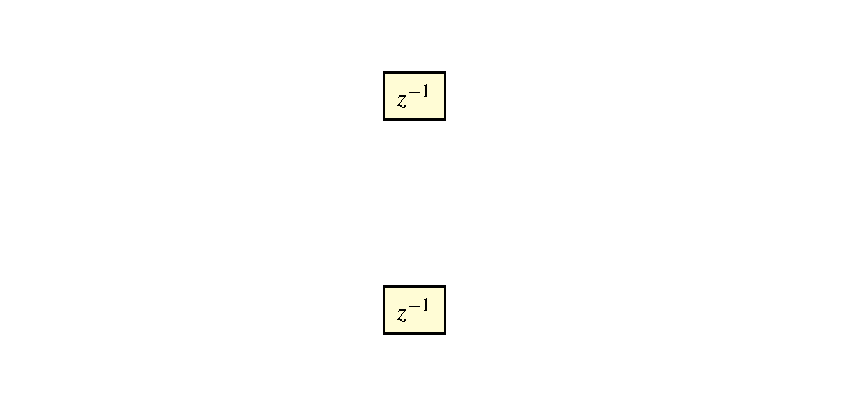
\includegraphics[width=0.85\columnwidth]{./Unit-03/img/PS01-ex02-fig01.pdf}
           \end{center}}
 \only<3 >{If the inputs are the $x_i(k+1)$, then the outputs are the $x_i(k)$:\\
           \begin{center}
            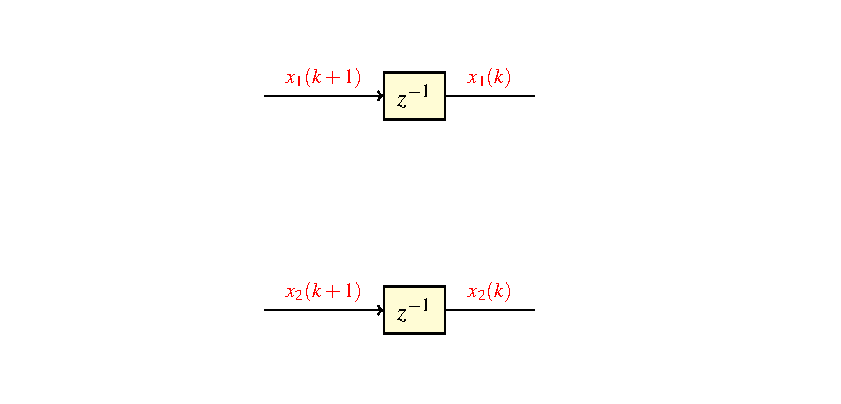
\includegraphics[width=0.85\columnwidth]{./Unit-03/img/PS01-ex02-fig02.pdf}
           \end{center}}
 \only<4 >{Now place the elements of \textcolor{magenta}{$A$} and \textcolor{blue}{$b$}:\\
           \begin{center}
            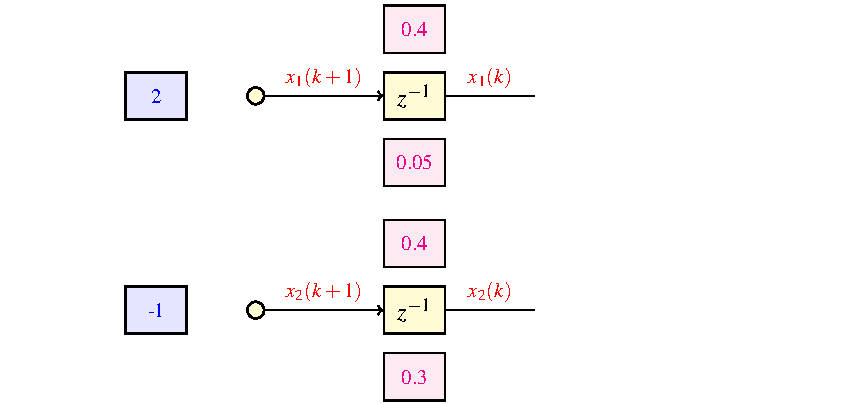
\includegraphics[width=0.85\columnwidth]{./Unit-03/img/PS01-ex02-fig03.pdf}
           \end{center}}
 \only<5 >{Read the state equation and wire how $x(k+1)$ depends on $x(k)$:\\
           \begin{center}
            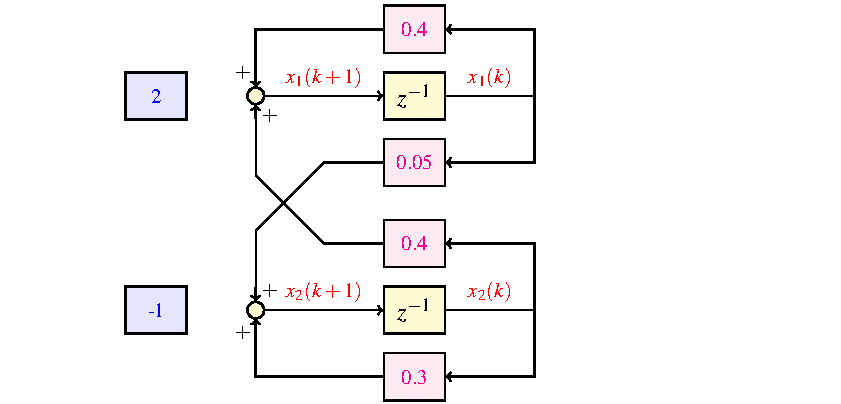
\includegraphics[width=0.85\columnwidth]{./Unit-03/img/PS01-ex02-fig04.pdf}
           \end{center}}
 \only<6 >{Continue reading and wire how $x(k+1)$ depends on $u(k)$:\\
           \begin{center}
            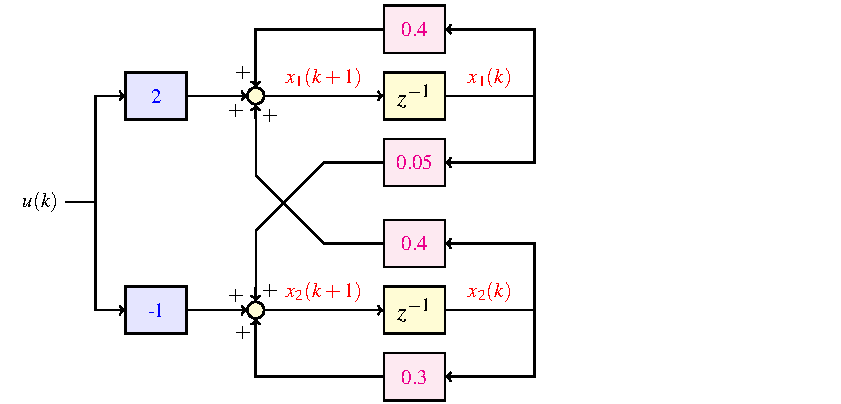
\includegraphics[width=0.85\columnwidth]{./Unit-03/img/PS01-ex02-fig05.pdf}
           \end{center}}
 \only<7 >{Now place the elements of \textcolor{green!80!black}{$c$}:\\
           \begin{center}
            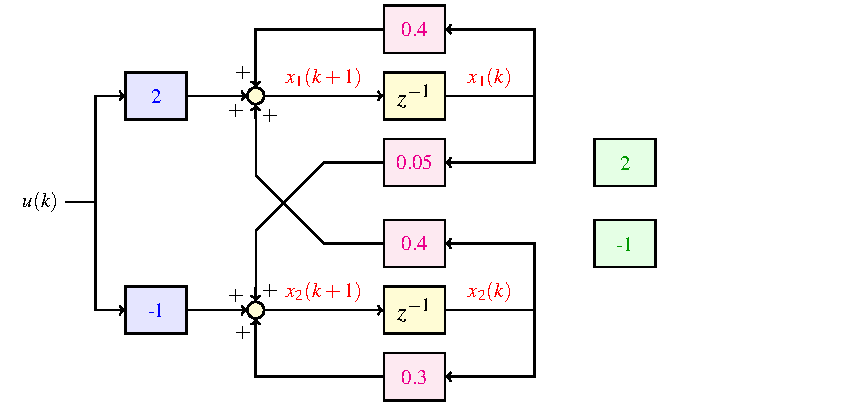
\includegraphics[width=0.85\columnwidth]{./Unit-03/img/PS01-ex02-fig06.pdf}
           \end{center}}
 \only<8->{Read the output equation and complete the block diagram:\\
           \begin{center}
            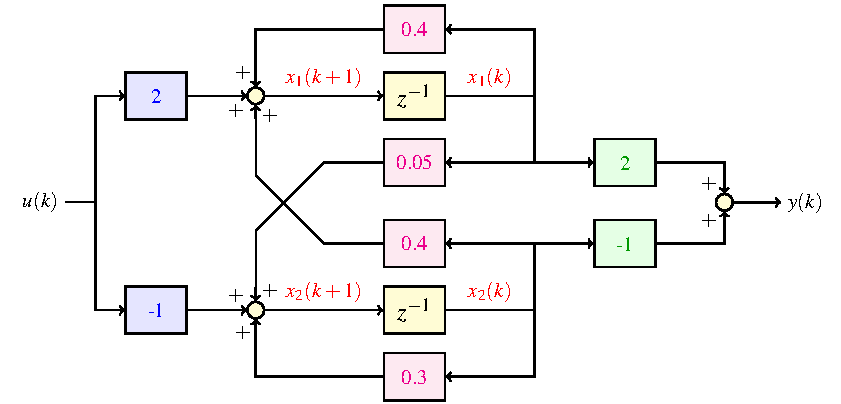
\includegraphics[width=0.85\columnwidth]{./Unit-03/img/PS01-ex02-fig07.pdf}
           \end{center}}
\end{frame}

\begin{frame}
\frametitleTC{Proposed exercise 02}
\framesubtitleTC{Try this at home, ask questions next time if needed}
\myPause
 Take the same system as in the previous proposed exercise, i.e.,
 \begin{displaymath}
  A = \begin{bmatrix} 0.5 & 0 \\ 2 & -0.3 \end{bmatrix}, \quad
  b = \begin{bmatrix} 1 \\ 0 \end{bmatrix}, \quad
  c = \begin{bmatrix} 0 & 4 \end{bmatrix}, \quad
  d = 1,
 \end{displaymath}
 and turn it into a block diagram.\\ \myPause
 \vspace{5mm}Remark: in this case you will see a \TC{direct feedthrough} from $u$ to $y$,\\
 because $d \neq 0$. 
\end{frame}

\begin{frame}
\frametitleTC{Takeaways}
\framesubtitleTC{from exercise 02 (and the proposed one)}
\myPause
 \begin{itemize}[<+-| alert@+>]
 \item Generalise the situation with compact matrix notation (thick lines are vectors):
       \begin{center}
        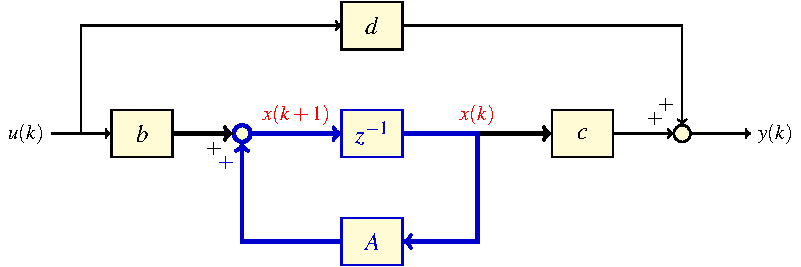
\includegraphics[width=0.65\columnwidth]{./Unit-03/img/PS01-ex02-takeaway-FBscheme.pdf}
       \end{center}
 \item Do you see the \textcolor{blue!80!black}{feedback loop} inherently inside the system?
 \item Feedback is not ``an invention for control''; it is an integral part\\
       of how nature works!
 \end{itemize}
\end{frame}

\begin{frame}
\frametitleTC{Takeaways}
\framesubtitleTC{from exercise 02 (and the proposed one)}
\myPause
 \begin{itemize}[<+-| alert@+>]
 \item Get acquainted with the $(k,k-1)$ and the $(k+1,k)$ ways of writing a DT system,\\
       and always pay attention to which symbol is what.
 \item In particular, the $u$ in the state equation is NOT at the same instant as that\\
       in the output equation, no matter how the system is written.
 \item \vspace{4mm}As feedback is a powerful weapon, ``slight'' approximations as taking\\
       the previous input of a block and not the current, or \emph{vice versa},\\
       can in fact be devastating...
 \item ...and without a system-theoretical analysis, this is impossible\\
       to figure out before the system is run --- i.e., possibly, broken.
 \end{itemize}
\end{frame}




\section{Exercise 03}
\subsection{}

\begin{frame}
\frametitleTC{Problem}
\framesubtitleTC{This one we solve together}
 Given the two DT LTI dynamic systems
 \begin{displaymath}
  S_1:
  \left\{\begin{array}{rcl}
   x_1(k) &=& 0.5x_1(k-1)+u(k-1)\\
   x_2(k) &=& 0.5x_2(k-1)+u(k-1)\\
   y(k)   &=& x_1(k)+x_2(k)
  \end{array}\right. \quad
  S_2:
  \left\{\begin{array}{rcl}
   x_1(k) &=& 0.4x_1(k-1)+u(k-1)\\
   x_2(k) &=& 0.8x_2(k-1)+u(k-1)\\
   y(k)   &=& x_2(k)
  \end{array}\right.
 \end{displaymath}

 \begin{itemize}[<+-| alert@+>]
 \item[(a)] compute their transfer functions,
 \item[(b)] comment on the result.
 \end{itemize}
\end{frame}

\begin{frame}
\frametitleTC{Solution}
\framesubtitleTC{Item (a)}
\myPause
 \begin{itemize}[<+-| alert@+>]
 \item We start with $S_1$:
       \begin{itemize}
       \item[] \begin{itemize}[<+-| alert@+>]
               \item[$G(z)$] \vspace{1mm}
                    $= \begin{bmatrix} 1 & 1  \end{bmatrix} \,
                       \begin{bmatrix} z-0.5 & 0 \\
                                       0     & z-0.5 \end{bmatrix}^{-1} \,
                       \begin{bmatrix} 1 \\ 1 \end{bmatrix}
                       +0
                    $
               \item[] \vspace{1mm}
                    $= \cfrac{1}{(z-0.5)^2}
                       \begin{bmatrix} 1 & 1 \end{bmatrix} \,
                       \begin{bmatrix} z-0.5 & 0 \\
                                       0     & z-0.5 \end{bmatrix} \,
                       \begin{bmatrix} 1 \\ 1 \end{bmatrix}
                    $
               \item[] \vspace{1mm}
                    $= \cfrac{1}{(z-0.5)^2}
                       \begin{bmatrix} z-0.5 & z-0.5 \end{bmatrix} \,
                       \begin{bmatrix} 1 \\ 1 \end{bmatrix}
                    $
               \item[] \vspace{1mm}
                    $= \cfrac{2\cancel{(z-0.5)}}{(z-0.5)^{\cancel{2}}} \qquad \qquad
                       \TC{\leftarrow \text{zero/pole \underline{cancellation}}}
                    $
               \item[] \vspace{1mm}
                    $= \cfrac{2}{z-0.5}.
                    $
               \end{itemize}
       \end{itemize}
 \end{itemize}
\end{frame}


\begin{frame}[fragile]
\frametitleTC{Solution}
\framesubtitleTC{Item (a)}
\myPause
 \begin{itemize}[<+-| alert@+>]
 \item And now $S_2$:
       \begin{itemize}
       \item[] \begin{itemize}[<+-| alert@+>]
               \item[] wxMaxima, we are lazy \smiley
                       \begin{verbatim}
A:matrix([0.4,0],[0,0.8]);
b:matrix([1],[1]);
c:matrix([0,1]);
G:c.invert(z*ident(2)-A).b;
                       \end{verbatim}
               \item[] \vspace{1mm}
                    $ G(z) = \cfrac{1}{z-0.8}.
                    $
               \end{itemize}
               \item \vspace{3mm}Another case with cancellation: the characteristic polynomial of $A$\\
                     has degree 2, the denominator of $G(z)$ has degree 1.
       \end{itemize}
 \end{itemize}
\end{frame}



\begin{frame}
\frametitleTC{Solution}
\framesubtitleTC{Item (b) -- comments on the $S_1$ case}
\myPause
 \begin{itemize}[<+-| alert@+>]
 \item In fact $S_1$ is a ``fake'' 2nd order system, since as far as induced motions are\\
       concerned  $x_1$ and $x_2$ are the same, and the system is \TC{input-output} (i.e, as far\\
       as we only look at $u$ and $y$) \TC{equivalent} to a 1st order one:
       \begin{displaymath}
        \left\{\begin{array}{rcl}
         x_1(k) &=& 0.5x_1(k-1)+u(k-1)\\
         x_2(k) &=& 0.5x_2(k-1)+u(k-1)\\
         y(k)   &=& x_1(k)+x_2(k)
        \end{array}\right. \quad
        \Rightarrow \quad
        \left\{\begin{array}{rcl}
         x(k) &=& 0.5x(k-1)+u(k-1)\\
         y(k) &=& 2x(k)
        \end{array}\right.
        \end{displaymath} 
        apparently with
        \begin{displaymath}
         G(z)=\cfrac{2}{z-0.5}.
        \end{displaymath} 
 \item This system cannot move in the whole $(x_1,x_2)$ plane, but only\\
       on the straight line $x_1=x_2$.
 \item In general, systems like this can only move on a \TC{subspace} (line)\\
       of their \TC{state space} (plane).
 \item We call them \TC{not fully reachable} (the term should be intuitive).
 \end{itemize}
\end{frame}

\begin{frame}
\frametitleTC{Solution}
\framesubtitleTC{Item (b) -- comments on the $S_2$ case}
\myPause
 \begin{itemize}[<+-| alert@+>]
 \item Also $S_2$ is a ``fake'' 2nd order system, because however $x_1$ moves, $y$ does not
       reveal this, and thus we can reduce this system as well to a 1st order one:
       \begin{displaymath}
        \left\{\begin{array}{rcl}
         x_1(k) &=& 0.4x_1(k-1)+u(k-1)\\
         x_2(k) &=& 0.8x_2(k-1)+u(k-1)\\
         y(k)   &=& x_2(k)
        \end{array}\right. \quad
        \Rightarrow \quad
        \left\{\begin{array}{rcl}
         x(k) &=& 0.8x(k-1)+u(k-1)\\
         y(k) &=& x(k)
        \end{array}\right.
        \end{displaymath} 
        apparently with
        \begin{displaymath}
         G(z)=\cfrac{1}{z-0.8}.
        \end{displaymath} 
 \item In this system one state variable does not influence the output.
 \item We call such systems \TC{not fully observable} (the term should be\\
       once again intuitive).
 \end{itemize}
\end{frame}

\begin{frame}
\frametitleTC{Proposed exercise 03}
\framesubtitleTC{Try this at home, ask questions next time if needed}
\myPause
 Take the two system of exercise 03, and turn them into block diagrams.\\
 \vspace{5mm}Analyse those diagrams along the idea that parts of the system are not influenced
 by the input, or do not influence the output. 
\end{frame}



\begin{frame}
\frametitleTC{Takeaways}
\framesubtitleTC{from exercise 03 (and the proposed one)}
\myPause
 \begin{itemize}[<+-| alert@+>]
 \item There are cases in which a system cannot move in all its state space, or equivalently,
       some state variables are not influenced by the input.
 \item Suggestion for reflections: why ``equivalently''?
 \item There are also cases in which some state variables do not influence the output.
 \item There are also cases where both facts occur.
 \item We detect this because in computing the transfer function we get\\
       \TC{cancellations}.
 \end{itemize}
\end{frame}

\begin{frame}
\frametitleTC{Takeaways}
\framesubtitleTC{from exercise 03 (and the proposed one)}
\myPause
 \begin{itemize}[<+-| alert@+>]
 \item Do we need to bother?
 \item Yes, because this collectively means that a system may have \TC{hidden parts}\\
       (things the transfer function does not tell).
 \item In setting up controls, we must be careful to not generate UNSTABLE hidden parts.
 \item We do not mind about asymptotically stable ones, because their effect\\
       vanishes with their free motion.
 \end{itemize}
\end{frame}




\section{Exercise 04}
\subsection{}

\begin{frame}[label={pag:ex-realisation}]
\frametitleTC{Problem}
\framesubtitleTC{This one we solve together}
\myPause
 Take the block diagram
 \begin{center}
  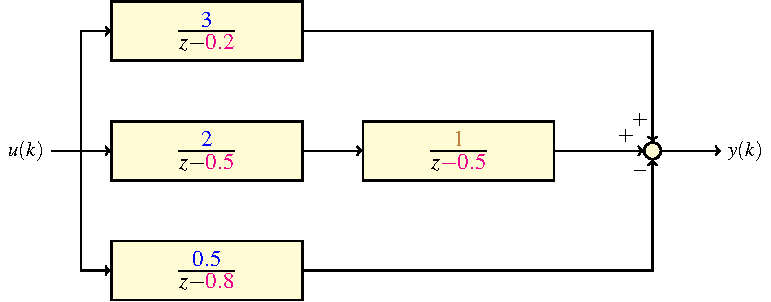
\includegraphics[width=0.85\columnwidth]{./Unit-03/img/PS01-ex04-fig01.pdf}
 \end{center}\myPause
 \begin{itemize}[<+-| alert@+>]
 \item[(a)] compute the transfer function from $u(k)$ to $y(k)$,
 \item[(b)] find a possible state-space description for the system.
 \end{itemize}
\end{frame}

\begin{frame}
\frametitleTC{Solution}
\framesubtitleTC{Item (a) -- preliminaries}
\myPause
 \begin{itemize}[<+-| alert@+>]
 \item Take two blocks in \TC{series} or \TC{cascade}, i.e., the output $y_1(k)$ of the first is the
       input $u_2(k)$ of the second. Name $G_1(z)$ and $G_2(z)$ their transfer functions.
 \item Let the overall system input $u(k)$ be connected to the input $u_1(k)$ of $G_1(z)$, and the overall
       system output $y(k)$ be the output $y_2(k)$ of $G_2(z)$.
 \item Then we have
       \begin{displaymath}
        y(k) = y_2(k) = G_2(z)u_2(k) = G_2(z)y_1(k) = G_2(z)G_1(z)u_1(k)=G_2(z)G_1(z)u(k),
       \end{displaymath}
 \item and therefore the overall transfer function $G(z)$ from $u(k)$ to $y(k)$ is
       \begin{displaymath}
        G(z) = G_2(z)G_1(z).
       \end{displaymath}
 \end{itemize}
\end{frame}

\begin{frame}
\frametitleTC{Solution}
\framesubtitleTC{Item (a) -- preliminaries}
\myPause
 \begin{itemize}[<+-| alert@+>]
 \item Take two blocks $G_1(z)$ and $G_2(z)$ in \TC{parallel}, i.e., they get the same input $u(k)$
       and their outputs sum together to produce the overall system output $y(k)$.
 \item With obvious notation have
       \begin{displaymath}
        y(k) = y_1(k)+y_2(k) = G_1(z)u_1(k)+G_2(z)u_2(k) = (G_1(z)+G_2(z))u(k),
       \end{displaymath}
 \item and therefore the overall transfer function $G(z)$ from $u(k)$ to $y(k)$ is
       \begin{displaymath}
        G(z) = G_1(z)+G_2(z).
       \end{displaymath}
 \item Extending to more blocks and different signs is trivial.
 \end{itemize}
\end{frame}

\begin{frame}
\frametitleTC{Solution}
\framesubtitleTC{Item (a)}
\myPause
 \begin{itemize}[<+-| alert@+>]
 \item The system under question is composed of three branches in parallel.
 \item The middle one is composed of two blocks in series.
 \item Hence (mind the signs) the overall transfer function $G(z)=y(k)/u(k)$ is
       \begin{displaymath}
        \begin{array}{rcll}
         G(z) &=& & \cfrac{3}{z-0.2}\\
              & &+& \cfrac{2}{z-0.5} \,\cdot\,
                    \cfrac{1}{z-0.5}\\
              & &-& \cfrac{0.5}{z-0.8} \; \ldots\\ \\
              &=& & \cfrac{2.5z^3-2.8z^2+0.925z-0.255}{(z-0.2)(z-0.5)^2(z-0.8)}.
        \end{array}
       \end{displaymath}
 \end{itemize}
\end{frame}

\begin{frame}
\frametitleTC{Solution}
\framesubtitleTC{Item (b)}
\myPause%
 \only<2 >{Consider the individual first-order blocks:\\%
           \begin{center}
            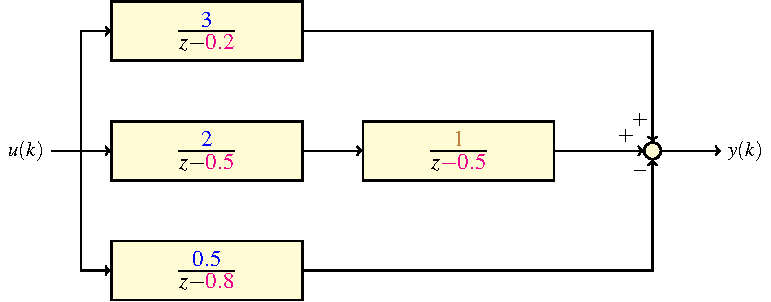
\includegraphics[width=0.85\columnwidth]{./Unit-03/img/PS01-ex04-fig01.pdf}
           \end{center}}
 \only<3 >{Take their outputs as state variables:\\%
           \begin{center}
            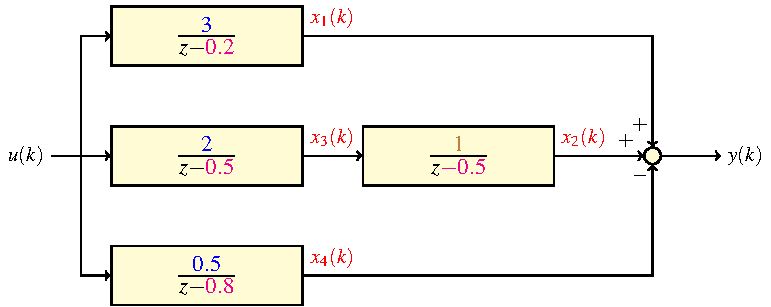
\includegraphics[width=0.85\columnwidth]{./Unit-03/img/PS01-ex04-fig02.pdf}
           \end{center}}
 \only<4->{write the elementary difference equations for each block:\\%
           \begin{center}
            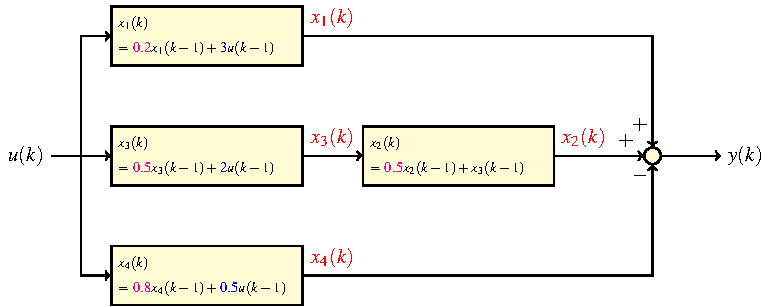
\includegraphics[width=0.85\columnwidth]{./Unit-03/img/PS01-ex04-fig03.pdf}
           \end{center}}
\end{frame}

\begin{frame}
\frametitleTC{Solution}
\framesubtitleTC{Item (b)}
\myPause
 \begin{itemize}[<+-| alert@+>]
 \item Now put it all together:
       \begin{displaymath}
        \left\{\begin{array}{rlllll}
         x_1(k) &= 0.2x_1(k-1) &              &              &              & +u(k-1)    \\
         x_2(k) &=             & +0.5x_2(k-1) & +x_3(k-1)                                \\
         x_3(k) &=             &              &  0.5x_3(k-1) &              & +2u(k-1)   \\
         x_4(k) &=             &              &              &  0.8x_4(k-1) & +0.5u(k-1) \\
         y(k)   &= x_1(k)      & +x_2(k)      &              & -x_4(k)                   \\
        \end{array}\right.
       \end{displaymath}
 \item Hence
       \begin{displaymath}
        \begin{array}{c}
         A = \begin{bmatrix}
              0.2 & 0   & 0   & 0   \\
              0   & 0.5 & 1   & 0   \\
              0   & 0   & 0.5 & 0   \\
              0   & 0   & 0   & 0.8
             \end{bmatrix}, \quad
         b = \begin{bmatrix} 1 \\ 0 \\ 2 \\ 0.5 \end{bmatrix}, \\ \\
         c = \begin{bmatrix} 1 & 0 & 1 & -1 \end{bmatrix}, \quad
         d = 0.
        \end{array}
       \end{displaymath}
 \end{itemize}
\end{frame}

\begin{frame}
\frametitleTC{Takeaways}
\framesubtitleTC{from exercise 04}
\myPause
 \begin{itemize}[<+-| alert@+>]
 \item We know that the poles of $G(z)$ are eigenvalues of $A$.
 \item Not THE eigenvalues, some may be cancelled.
 \item Our matrices are real, hence eigenvalues (and poles) are either real, or in complex
       conjugate couples. Here we limit the math to real ones (but results hold in general).
 \item \vfill It should be clear that \emph{any} $G(z)$, once decomposed in simple fractions,\\
       can be treated as we did.
 \item Can we say something on our $A$? Can we use it to understand\\
       the eigenvalues--stability relationship we mentioned? 
 \item Remember that the free motion of a system converges to zero,\\
       diverges or neither, if so  does $A^k$ for $k\rightarrow\infty$. Let us have a look\\
       with this idea in mind.
 \end{itemize}
\end{frame}

\begin{frame}
\frametitleTC{Takeaways}
\framesubtitleTC{from exercise 04}
\myPause
 \begin{itemize}[<+-| alert@+>]
 \item In general, once treated as we did, matrix $A$ looks e.g. as follows:
 \begin{displaymath}
  A = 
  \begin{bmatrix}
   \-& \cellcolor{green!30!white}{\lambda_{1}} & 0 & 0 & 0 & 0 & 0 & 0 & \ldots & \\
   \-& 0 &\cellcolor{green!30!white}{\lambda_{2}}  & 0 & 0 & 0 & 0 & 0 \\
   \-& 0 & 0 &\cellcolor{orange!50!white}{\lambda_{3}}
             &\cellcolor{yellow!30!white}{\textcolor{cyan!80!black}{0}} & 0 & 0 & 0 \\
   \-& 0 & 0 &\cellcolor{yellow!30!white}{0}
             &\cellcolor{orange!50!white}{\lambda_{3}} & 0 & 0 & 0 \\
   \-& 0 & 0 & 0 & 0 &\cellcolor{orange!50!white}{\lambda_{4}}
                     &\cellcolor{orange!30!white}{\textcolor{red}{1}} & \cellcolor{yellow!30!white}{0} \\
   \-& 0 & 0 & 0 & 0 &\cellcolor{orange!30!white}{0}
                     &\cellcolor{orange!50!white}{\lambda_{4}}
                     & \cellcolor{yellow!30!white}{\textcolor{cyan!80!black}{0}} \\
   \-& 0 & 0 & 0 & 0 &\cellcolor{yellow!30!white}{0}
                     &\cellcolor{yellow!30!white}{0} & \cellcolor{orange!50!white}{\lambda_{4}} \\
   \-& \vdots &&&&&&& \ddots \\
  \end{bmatrix}
 \end{displaymath}
 \item Notice the block diagonal structure:
       \begin{itemize}[<+-| alert@+>]
       \item \colorbox{green!30!white}{single} eigenvalues are just diagonal elements;
       \item \colorbox{orange!50!white}{multiple} ones are repeated to form square \colorbox{yellow!30!white}{blocks},
       \item in turn diagonally composed of \colorbox{orange!30!white}{mini-blocks} separated by
             \textcolor{cyan!80!black}{zeroes}\\
             that break the over-diagonal sequence of \textcolor{red}{ones} in the block.
       \end{itemize}
 \end{itemize}
\end{frame}

\begin{frame}
\frametitleTC{Takeaways}
\framesubtitleTC{from exercise 04}
\myPause
 \begin{itemize}[<+-| alert@+>]
 \item Now, let us compute $A^k$:\myPause
 \begin{displaymath}
  A^k = 
  \begin{bmatrix}
   \-& \cellcolor{green!30!white}{\lambda_{1}^k} & 0 & 0 & 0 & 0 & 0 & 0 & \ldots & \\
   \-& 0 &\cellcolor{green!30!white}{\lambda_{2}^k}  & 0 & 0 & 0 & 0 & 0 \\
   \-& 0 & 0 &\cellcolor{orange!50!white}{\lambda_{3}^k}
             &\cellcolor{yellow!30!white}{\textcolor{cyan!80!black}{0}} & 0 & 0 & 0 \\
   \-& 0 & 0 &\cellcolor{yellow!30!white}{0}
             &\cellcolor{orange!50!white}{\lambda_{3}^k} & 0 & 0 & 0 \\
   \-& 0 & 0 & 0 & 0 &\cellcolor{orange!50!white}{\lambda_{4}^k}
                     &\cellcolor{orange!30!white}{\textcolor{red}{k\lambda_4^{k-1}}} & \cellcolor{yellow!30!white}{0} \\
   \-& 0 & 0 & 0 & 0 &\cellcolor{orange!30!white}{0}
                     &\cellcolor{orange!50!white}{\lambda_{4}^k}
                     & \cellcolor{yellow!30!white}{\textcolor{cyan!80!black}{0}} \\
   \-& 0 & 0 & 0 & 0 &\cellcolor{yellow!30!white}{0}
                     &\cellcolor{yellow!30!white}{0} & \cellcolor{orange!50!white}{\lambda_{4}^k} \\
   \-& \vdots &&&&&&& \ddots \\
  \end{bmatrix}
 \end{displaymath}\myPause
 \item Does it converge to a matrix of zeroes? Or diverge --- i.e., does\\
       at least one element diverge? Or neither?
 \item In other words, is the system asymptotically stable, unstable,\\
       or (simply) stable?
 \end{itemize}
\end{frame}

\begin{frame}[fragile]
\frametitleTC{Takeaways}
\framesubtitleTC{from exercise 04}
\myPause
 \begin{itemize}[<+-| alert@+>]
 \item Diagonal terms, in the form $\lambda^k$:
       \begin{displaymath}
        \begin{array}{rcl}
         \lim\limits_{k\rightarrow\infty}|\lambda^k| = 
          \begin{cases}
           0        & |\lambda| < 1 \\
           1        & |\lambda| = 1 \\
           \infty   & |\lambda| > 1 \\
          \end{cases}
        \end{array}
       \end{displaymath}
 \item Over-diagonal terms, in the form $k\lambda^k$:
       \begin{displaymath}
        \begin{array}{rcl}
         \lim\limits_{k\rightarrow\infty}|k\lambda^k| = 
          \begin{cases}
           0        & |\lambda| < 1 \\
           \infty   & |\lambda| \geq 1 \\
          \end{cases}
        \end{array}
       \end{displaymath}
 \item NOTE: larger mini-blocks give over-diagonal terms in other forms,\\
       but analogous as for the above. Take wxMaxima and try e.g.\\
       {\small
       \begin{verbatim}
  A:matrix([lambda,1,0],[0,lambda,1],[0,0,lambda]);
  A.A.A; /* NOT A^3, that is the elem-by-elem power */
       \end{verbatim}
       }
 \end{itemize}
\end{frame}

\begin{frame}
\frametitleTC{Takeaways}
\framesubtitleTC{from exercise 04}
\myPause
 \begin{itemize}[<+-| alert@+>]
 \item Now let us put it all together:
       \begin{itemize}[<+-| alert@+>]
       \item each single eigenvalue $\lambda_i$ only gives one diagonal term $\lambda_i^k$;
       \item each eigenvalue $\lambda_j$ with multiplicity $n_j$ gives $n_j$ diagonal terms $\lambda_j^k$, plus some\\
             \vspace{-0.75mm}over-diagonal terms $k\lambda_j^k$ -- or analogous -- iff the maximum size of its mini-block\\
             is greater then one.
       \end{itemize}
 \item Hence\\
       {\scriptsize 
       %\begin{center}
        \begin{tabular}{rcl}
         all $|\lambda_i|<1$                             & $\Rightarrow$ & System asymptotically stable\\
         \\
         at least one $|\lambda_i|>1$                    & $\Rightarrow$ & System unstable\\
         \\
         all $|\lambda_i|\leq 1$                         & \\
         and at least one has unity magnitude            & $\Rightarrow$ & System (simply) stable\\
         but in this case also unity max mini-block size & \\
         \\
         otherwise (i.e.,all $|\lambda_i|\leq 1$, and    & \\
         at least one has both unity magnitude and       & $\Rightarrow$ & System unstable\\
         maximum mini-block size greater than one)       & \\
        \end{tabular}
       %\end{center}
       }
 \item \vfill This proves (and completes) the statement of slide~\ref{pag:stab-eivals}.
 \end{itemize}
\end{frame}

 


\section{Wrap-up}
\subsection{}

\begin{frame}
\frametitleTC{Ideas and capabilities to take home}
\framesubtitleTC{(1/2) not necessarily in the same order as we saw them...}
 \begin{itemize}[<+-| alert@+>]
 \item Interpreting the state space description of a DT LTI dynamic system\\
       as scalar equations.
 \item Computing a system's transfer function from its state space description.
 \item Computing state and output responses in the time domain, and distinguishing\\
       free and induced motion.
 \item Commonly used signals: impulse, step, ramp.
 \end{itemize}
\end{frame}

\begin{frame}
\frametitleTC{Ideas and capabilities to take home}
\framesubtitleTC{(2/2)}
 \begin{itemize}[<+-| alert@+>]
 \item Poles and zeroes of a transfer functions, the former being eigenvalues\\
       of the dynamic matrix.
 \item Pole/zero cancellations and hidden parts.
 \item Writing a dynamic system as block diagram and recognise the inherent\\
       feedback in it.
 \item Combining blocks into overall transfer functions: for the moment series and parallel, more
       on this subject later on.
 \item A possible way to transform a transfer function into a state space\\
       representation.
 \item Stability and eigenvalues of the dynamic matrix (for the curious,\\
       we proved our statement by writing that matrix in \TC{Jordan} form).
 \end{itemize}
\end{frame}


